\documentclass{article}

% if you need to pass options to natbib, use, e.g.:
%     \PassOptionsToPackage{numbers, compress}{natbib}
% before loading neurips_2019

% ready for submission
% \usepackage{neurips_2019}

% to compile a preprint version, e.g., for submission to arXiv, add add the
% [preprint] option:
%     \usepackage[preprint]{neurips_2019}

% to compile a camera-ready version, add the [final] option, e.g.:
     \usepackage[final]{neurips_2019}

% to avoid loading the natbib package, add option nonatbib:
%     \usepackage[nonatbib]{neurips_2019}

\usepackage[utf8]{inputenc} % allow utf-8 input
\usepackage[T1]{fontenc}    % use 8-bit T1 fonts
\usepackage{hyperref}       % hyperlinks
\usepackage{url}            % simple URL typesetting
\usepackage{booktabs}       % professional-quality tables
\usepackage{amsfonts}       % blackboard math symbols
\usepackage{nicefrac}       % compact symbols for 1/2, etc.
\usepackage{microtype}      % microtypography
\usepackage{graphicx}

\title{Comparison of Dimensionality Reduction Techniques}

\author{%
  Jonathan Tan \\
  Harris School of Public Policy\\
  University of Chicago\\
  Chicago, IL 60637 \\
  \texttt{jonathantan@uchicago.edu} \\
  \And
  Satej Soman \\
  Harris School of Public Policy\\
  University of Chicago\\
  Chicago, IL 60637 \\
  \texttt{satej@uchicago.edu} \\
}

\begin{document}

\maketitle

\begin{abstract}
  We compare two dimensionality-reduction techniques: principle components analysis (PCA) and latent space representation via autoencoder neural networks. Both techniques are applied to a feature set and the reduced feature-set is used as the independent variables in a linear regression to recover a known score. We find that autoencoders with sigmoid activations outperform both PCA and ReLU-activation neural networks for this dimensionality reduction task. 
\end{abstract}

\section{Background}
Dimensionality reduction is an important technique to render high-dimensional datasets more tractable for analysis. Often, in a dataset containing thousands of columns, a small number of those columns are relevant for an analytical task. Robust techniques for identifying the most salient features allow for more compact representations of data, reducing storage costs and analysis time [1], [2].

\section{Techniques studied}
\subsection{Principal components analysis}
Principal component analysis is a dimensionality reduction technique built upon the singular value decomposition (SVD) of a feature matrix. Specifically, the SVD produces matrices $X = U \Sigma V^T$ such that the right singular vectors of $X$, i.e. the columns of $V$, give the principal component directions of $X$. We can obtain a lower-dimensional representation of the original features by projecting the data onto the first $n$ principal component directions. [3] Below, we vary the number of principal components used to predict wine scores and observe how mean squared error between predicted and true wine scores vary with $n$.

A known limitation of PCA is that it is not particularly effective at detecting and representing nonlinear relationships in the data. Thus, we are interested in exploring dimensionality reduction techniques that address this limitation.
\subsection{Autoencoders}
In contrast, autoencoders seek to map inputs to a \emph{non-linear} input manifold. An autoencoder is an artificial neural network that seeks to learn a compressed representation of its input [1], [4], [5]. Generally, an autoencoder has two stages: a number of encoding layers that reduce the dimension of the input vectors, and a number of decoding layers that attempt to reconstruct the original input from the latent representation. Our networks focus on the encoding step since we are interested in the latent representation.

All of our autoencoders produced output vectors of length 50. We trained neural networks with three main architectures. The shallowest was simply a 50-layer hidden layer in between an input and output layer. The deeper networks we tested progressively stepped the input size down. Most of our architectures had only a single decoding layer. We also tested networks where all layers had the same activation function (either sigmoid or ReLU), as well as an architecture where all hidden and input layers had ReLU activation, feeding into an output layer with sigmoid activation.

To train the networks, we used stochastic gradient descent over a variable number of training epochs. To maintain decoded fidelity, our output node delta for the update step was proportional to the difference in input and output vectors [6].
\section{Dataset}
\subsection{Description}
We use a dataset of wine reviews from Kaggle [7] consisting mostly of categorical and text data, each with an associated wine review score on a scale of 80 - 100. The features include a free-text description of the wine, as well as pre-parsed information about the wine, including type, grape variety, region of origin, and winery. The key continuous, numeric column in the feature set is the price of each wine bottle. The label we seek to recover is the wine review score.

\subsection{Preprocessing}
Much of the Kaggle dataset is text or categorical data. Specifically, the “description” feature contains paragraph text of descriptors for each wine. To obtain a numeric representation of this text data, we used a simple boolean bag-of-words model. We first preprocessed the text data by converting all words to lowercase, removing non-alphanumeric characters and common stopwords, then tokenizing the space-delimited string into separate words. Lastly, we computed a bit vector for each row that represented a one-hot encoding for each word in the description, over all unique words in all rows of the description feature.

The bag-of-words model gives a particularly sparse matrix, and we faced initial difficulties in computing the representation with the full 130,000-row dataset (which had roughly 45,000 unique tokens). Specifically, the resulting matrix from the description column alone was over 100GB and, when the process ran in a reasonable amount of time, we had difficulty storing the data on our local machines. As an interim solution, we proceeded with a reduced dataset, taking 10,000 rows from the wine dataset instead. 

In the future, other numeric representations of text data could be interesting to explore, e.g. low-dimensional word embeddings produced by neural network-based algorithms such as \verb+word2vec+ or \verb+GloVe+. [8] 

\section{Methodology}
For each technique, we apply the dimensionality reduction to obtain a reduced set of feature vectors ($X_j$). We then regress wine score ($S_i$) on these reduced features to estimate the least squares weights for the reduced feature set and then calculate predicted scores from the learned weights. Finally, we compare the mean-squared error arising from the true vs. predicted wine scores for several dimensionality reduction techniques.

\section{Results}
Table \ref{msetable} shows the resulting mean-squared errors for each dimensionality technique we studied, along with a description of each technique. For PCA runs, we report the number of principal components used in regression. For autoencoders, we report the architecture (shallow: 1 hidden layer, medium: 3 hidden layers, deep: 5 hidden layers), the activation function (ReLU or sigmoid), and the number of epochs used to train the network. There are two special networks: one ReLU network with a sigmoid output layer, and a completely symmetric network with the same number of encoding and decoding layers. 

As the table indicates, the sigmoid autoencoder performed the best, followed by PCA with a reasonable number of components, and then ReLU autoencoders. The special architectures described above did not improve performance.

Figures \ref{msek}, \ref{aenn_sigmoid}, and \ref{aenn_relu} investigate the performance of each technique in more detail. As seen in Figure \ref{msek}, MSE drops very quickly as the number of included principle components increases but levels off after approximately 5 or so included components. This indicates the ideal \emph{linear} representation of the data is captured by those components.

Figures \ref{aenn_sigmoid} and \ref{aenn_relu} look at the neural networks' performance. Surprisingly, the number of epochs we trained the network for had no effect on MSE. Additionally, the shallow architectures outperformed the deeper ones, while sigmoid activation was orders of magnitude more performant than ReLU activation.

\begin{table}
    \centering\small
\begin{tabular}{llr}
\toprule
     technique &                     description &          MSE \\
\midrule
autoencoder &   sigmoid, shallow, 1000 epochs &     5.649318 \\
autoencoder &  sigmoid, shallow, 10000 epochs &     5.649318 \\
autoencoder &     sigmoid, shallow, 10 epochs &     5.649318 \\
autoencoder &    sigmoid, shallow, 100 epochs &     5.649318 \\
autoencoder &  sigmoid, symmetric, 100 epochs &     5.653316 \\
autoencoder &    sigmoid, medium, 1000 epochs &     5.653316 \\
autoencoder &      sigmoid, medium, 10 epochs &     5.653316 \\
autoencoder &     sigmoid, medium, 100 epochs &     5.653316 \\
autoencoder &   sigmoid, medium, 10000 epochs &     5.653316 \\
autoencoder &     sigmoid, deep, 10000 epochs &     5.665386 \\
autoencoder &      sigmoid, deep, 1000 epochs &     5.665386 \\
autoencoder &       sigmoid, deep, 100 epochs &     5.665386 \\
autoencoder &        sigmoid, deep, 10 epochs &     5.665386 \\
        PCA &                  100 components &   231.751525 \\
        PCA &                   50 components &   307.355949 \\
        PCA &                   25 components &   366.782639 \\
        PCA &                   20 components &   399.109070 \\
        PCA &                   15 components &   412.171071 \\
        PCA &                   10 components &   426.216375 \\
        PCA &                    5 components &   481.270942 \\
        PCA &                    3 components &   484.869192 \\
        PCA &                    2 components &   516.873620 \\
autoencoder &        ReLU, deep, 10000 epochs &  1074.289408 \\
autoencoder &         ReLU, deep, 1000 epochs &  1074.289408 \\
autoencoder &          ReLU, deep, 100 epochs &  1074.289408 \\
autoencoder &           ReLU, deep, 10 epochs &  1074.289408 \\
autoencoder &        ReLU, shallow, 10 epochs &  1732.283164 \\
autoencoder &       ReLU, shallow, 100 epochs &  1732.283164 \\
autoencoder &      ReLU, shallow, 1000 epochs &  1732.283164 \\
autoencoder &     ReLU, shallow, 10000 epochs &  1732.283164 \\
autoencoder &      ReLU, medium, 10000 epochs &  1742.411749 \\
autoencoder &       ReLU, medium, 1000 epochs &  1742.411749 \\
autoencoder &        ReLU, medium, 100 epochs &  1742.411749 \\
autoencoder &         ReLU, medium, 10 epochs &  1742.411749 \\
autoencoder &    ReLU, sigmoidOut, 100 epochs &  1742.411749 \\
        PCA &                    1 components &  4524.018520 \\
\bottomrule
\end{tabular}
\caption{Mean-squared error results for various dimensionality reduction techniques.}
\label{msetable}
\end{table}

\begin{figure}
\centering
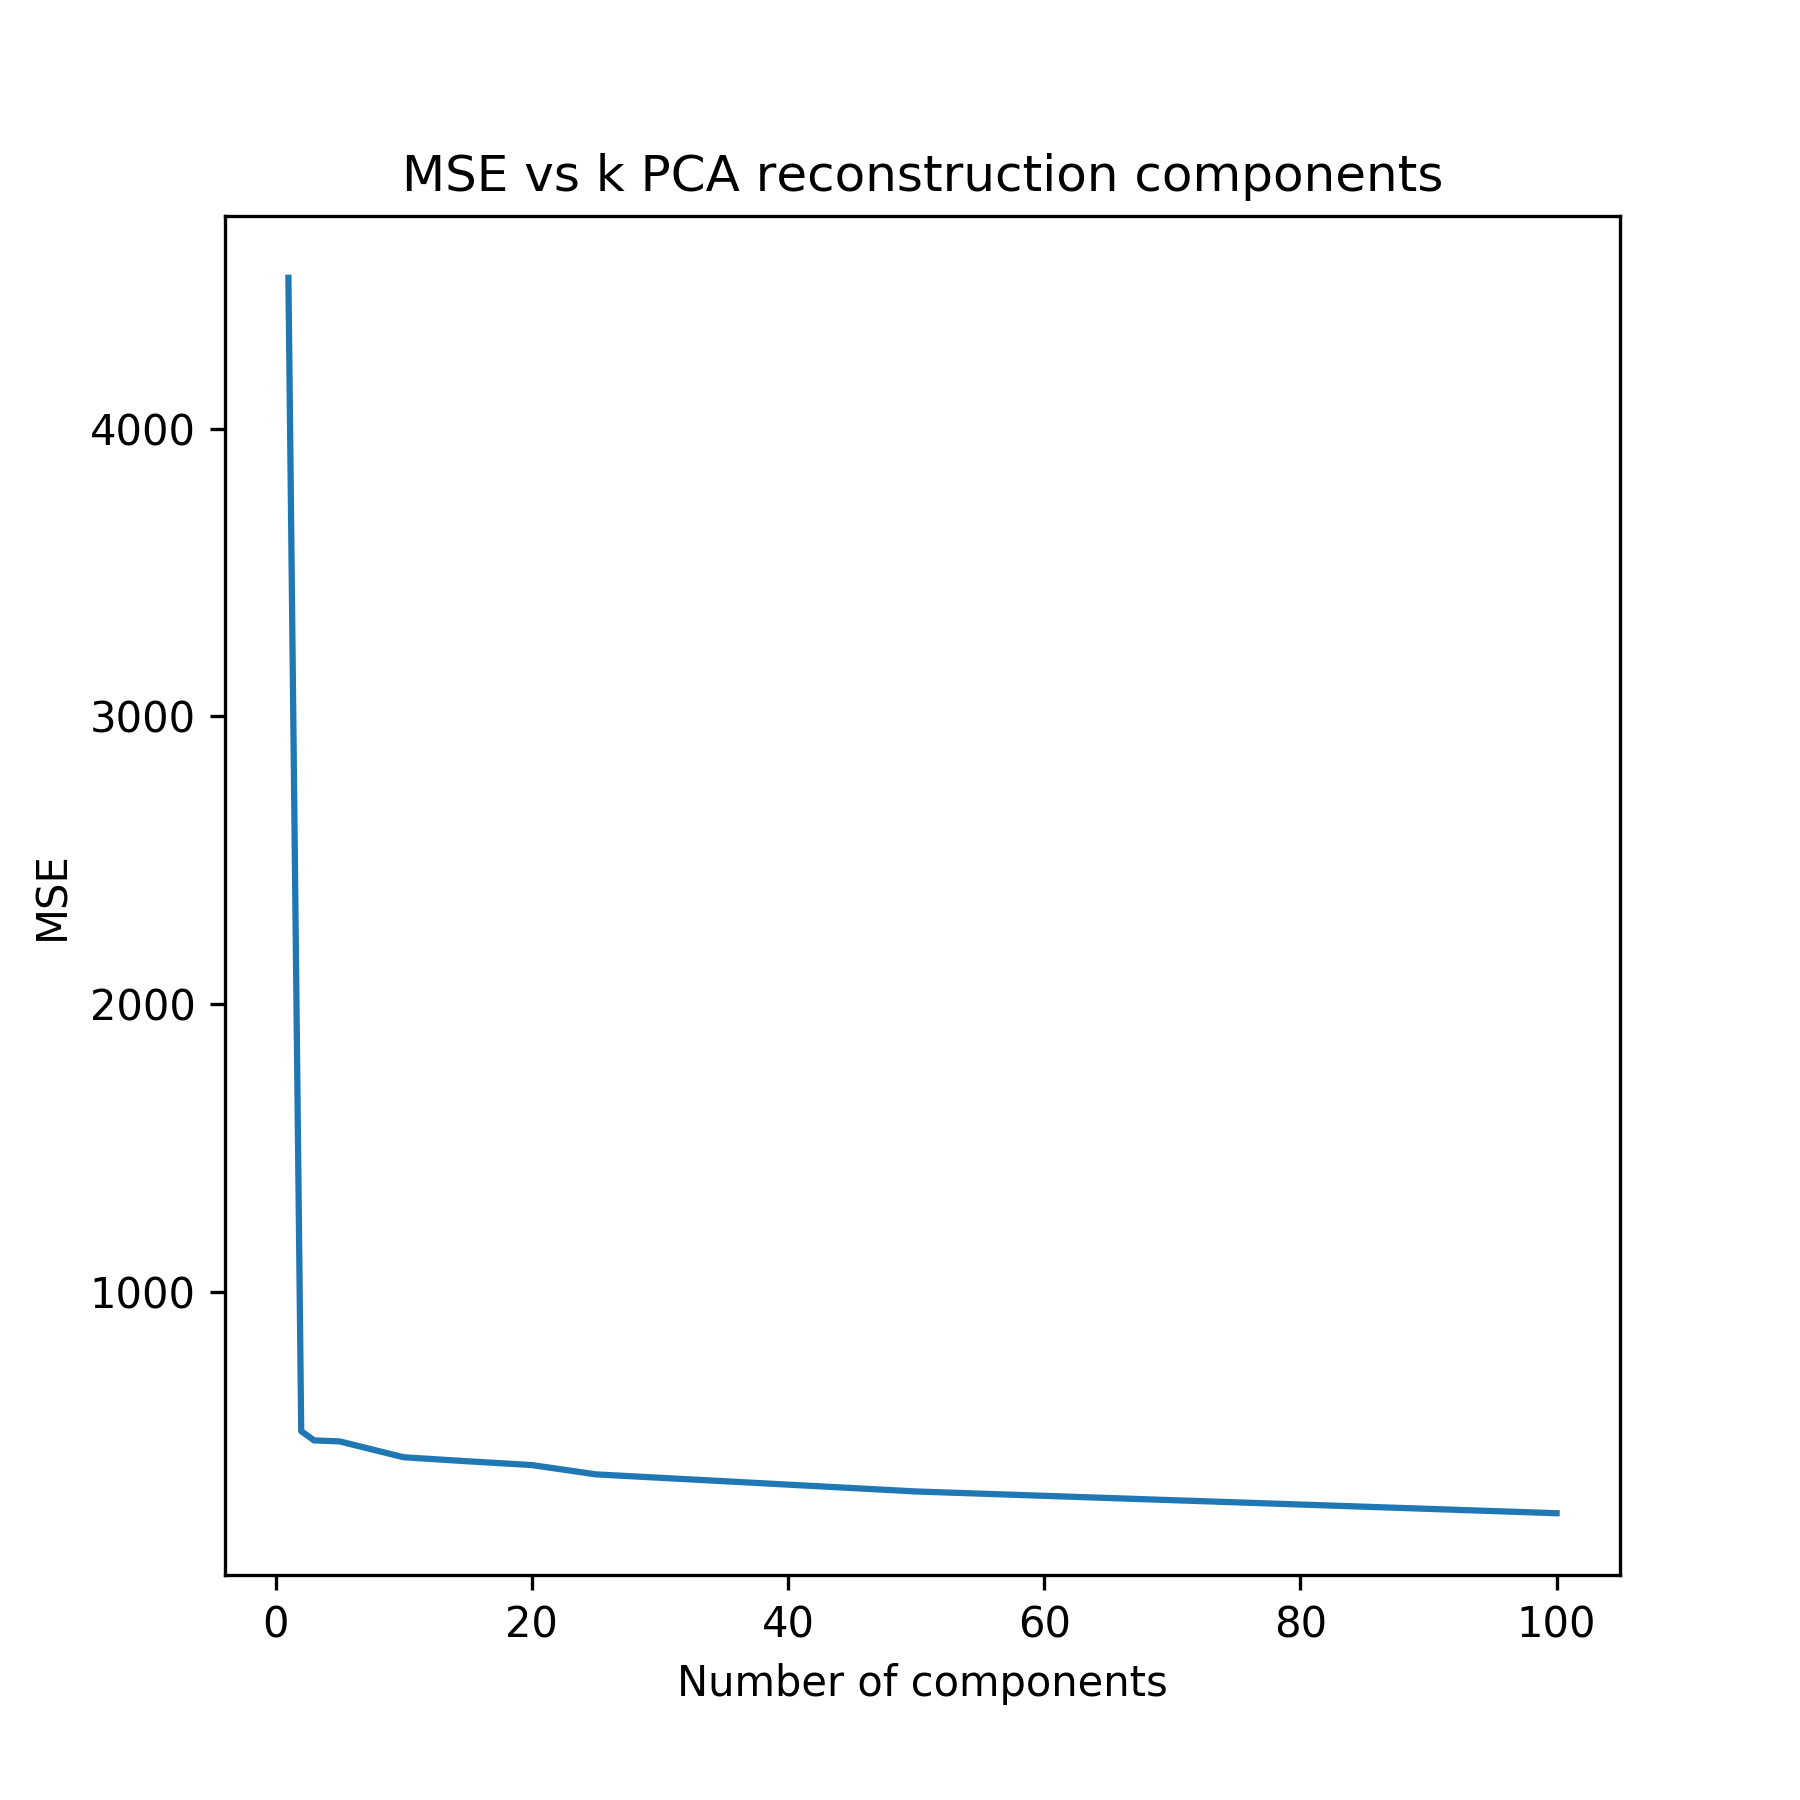
\includegraphics[width=0.7\textwidth]{../images/pca_mse_vs_k.png}
\caption{Mean-square error of PCA as number of principle components included increases.}
\label{msek}
\end{figure}

\begin{figure}
\centering
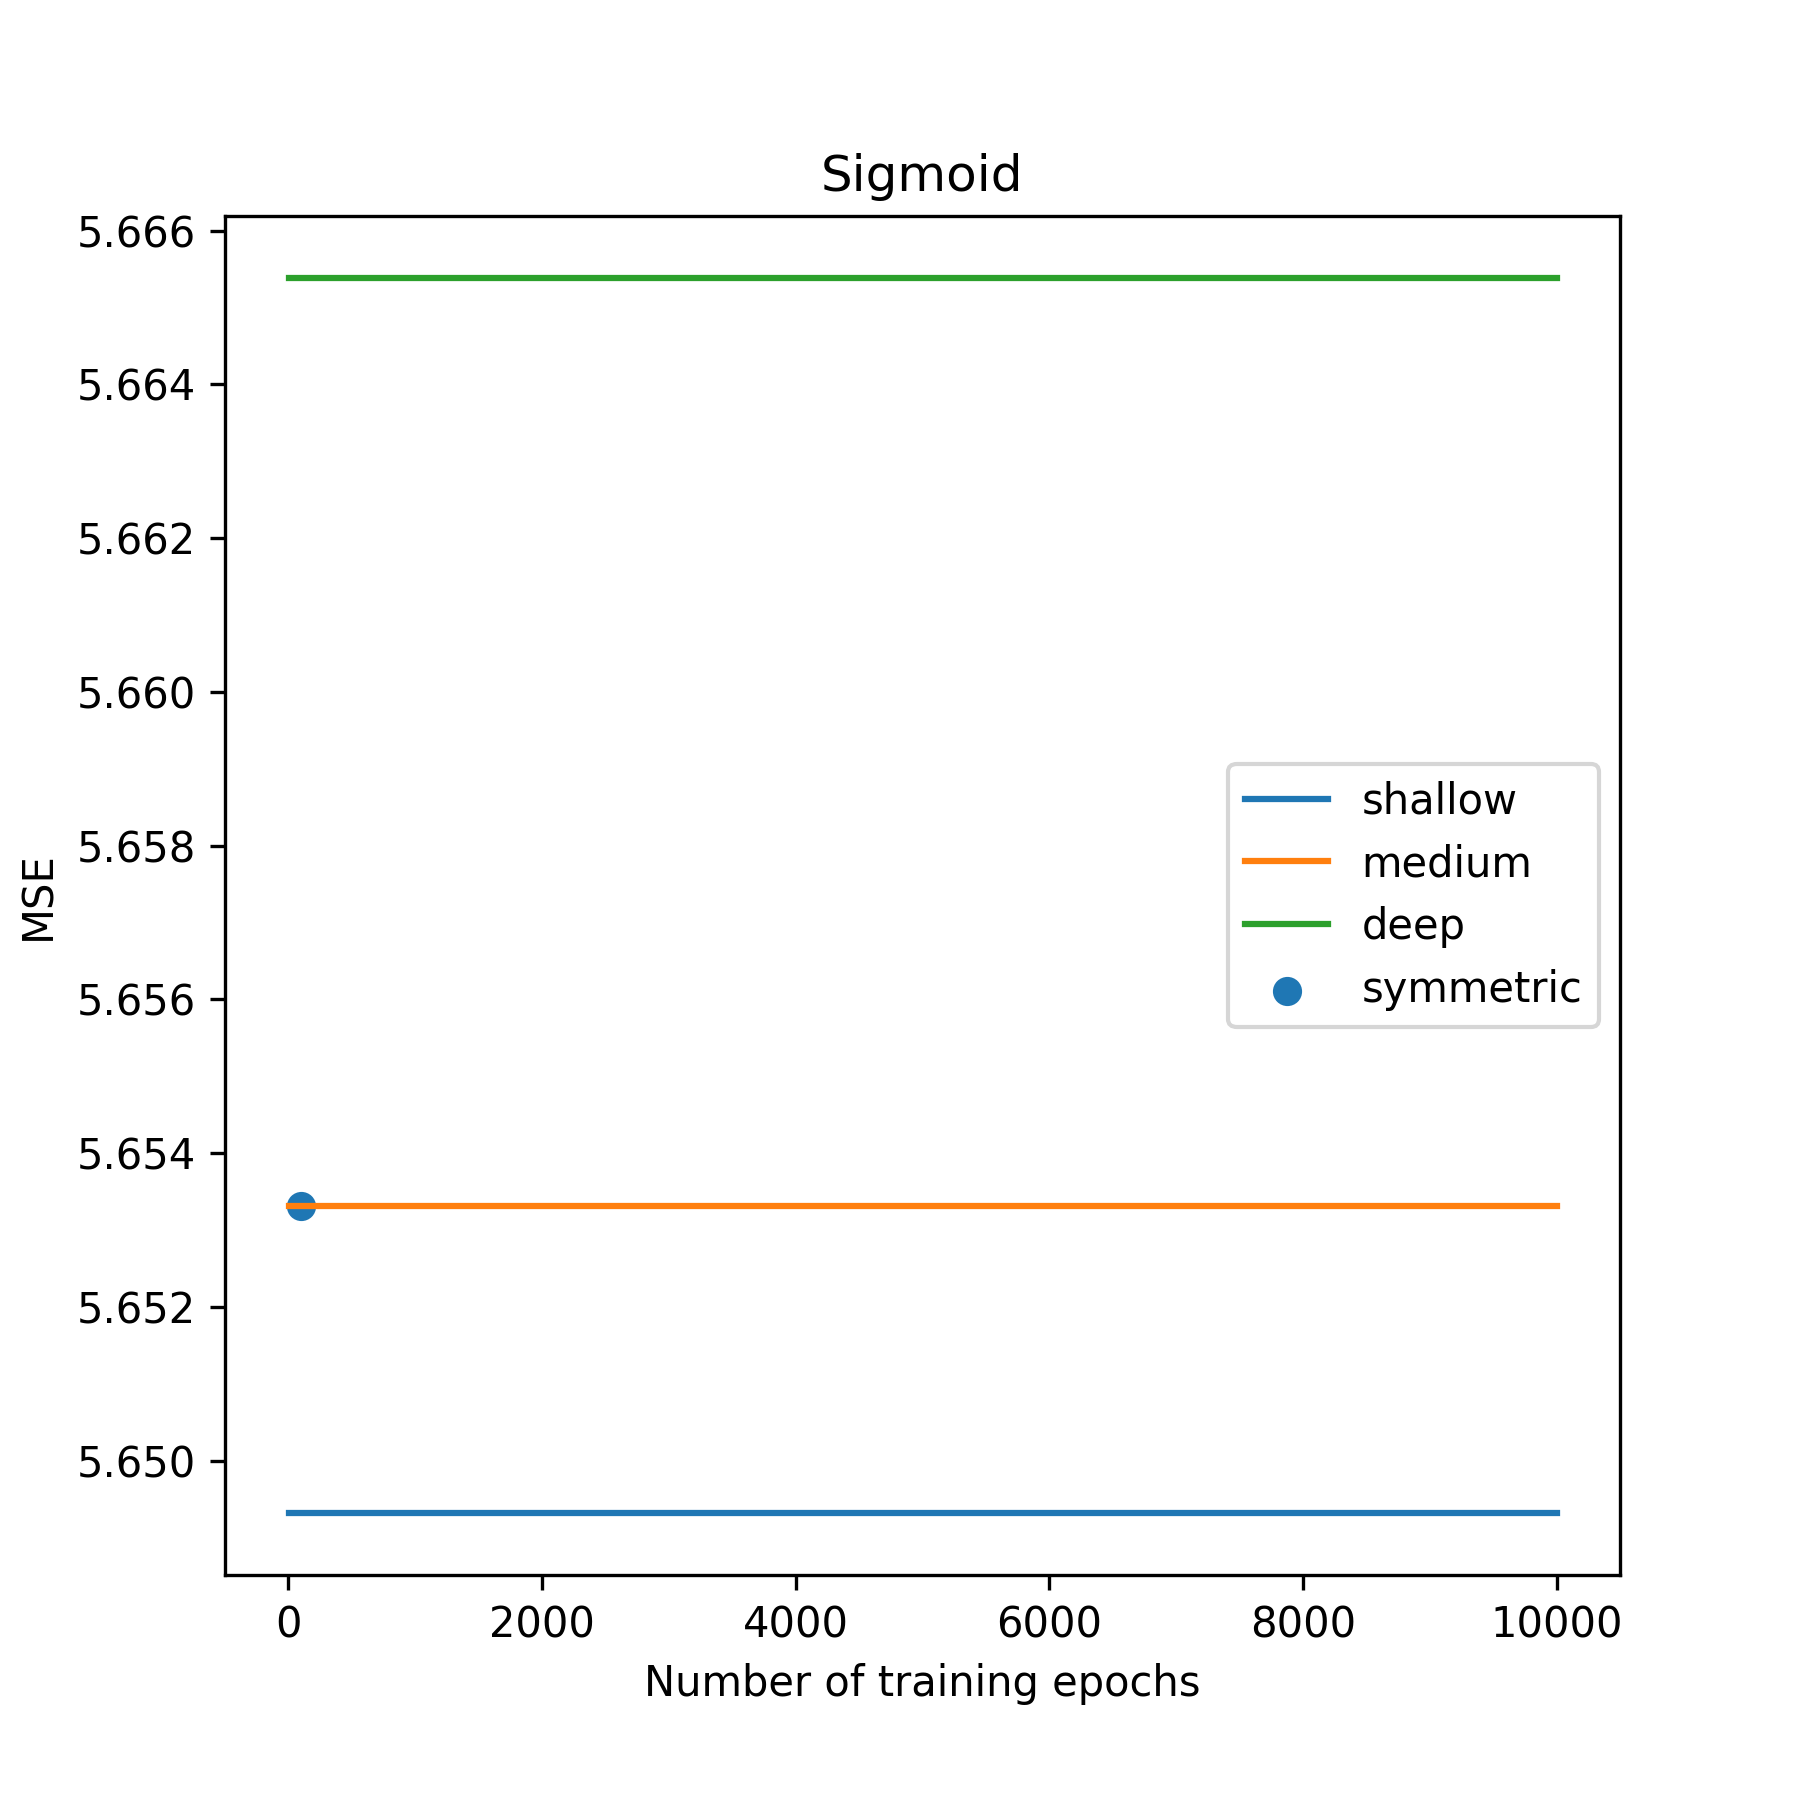
\includegraphics[width=0.7\textwidth]{../images/aenn_results_sigmoid.png}
\caption{Mean-square error of sigmoid activation AENN across training periods.}
\label{aenn_sigmoid}
\end{figure}

\begin{figure}
\centering
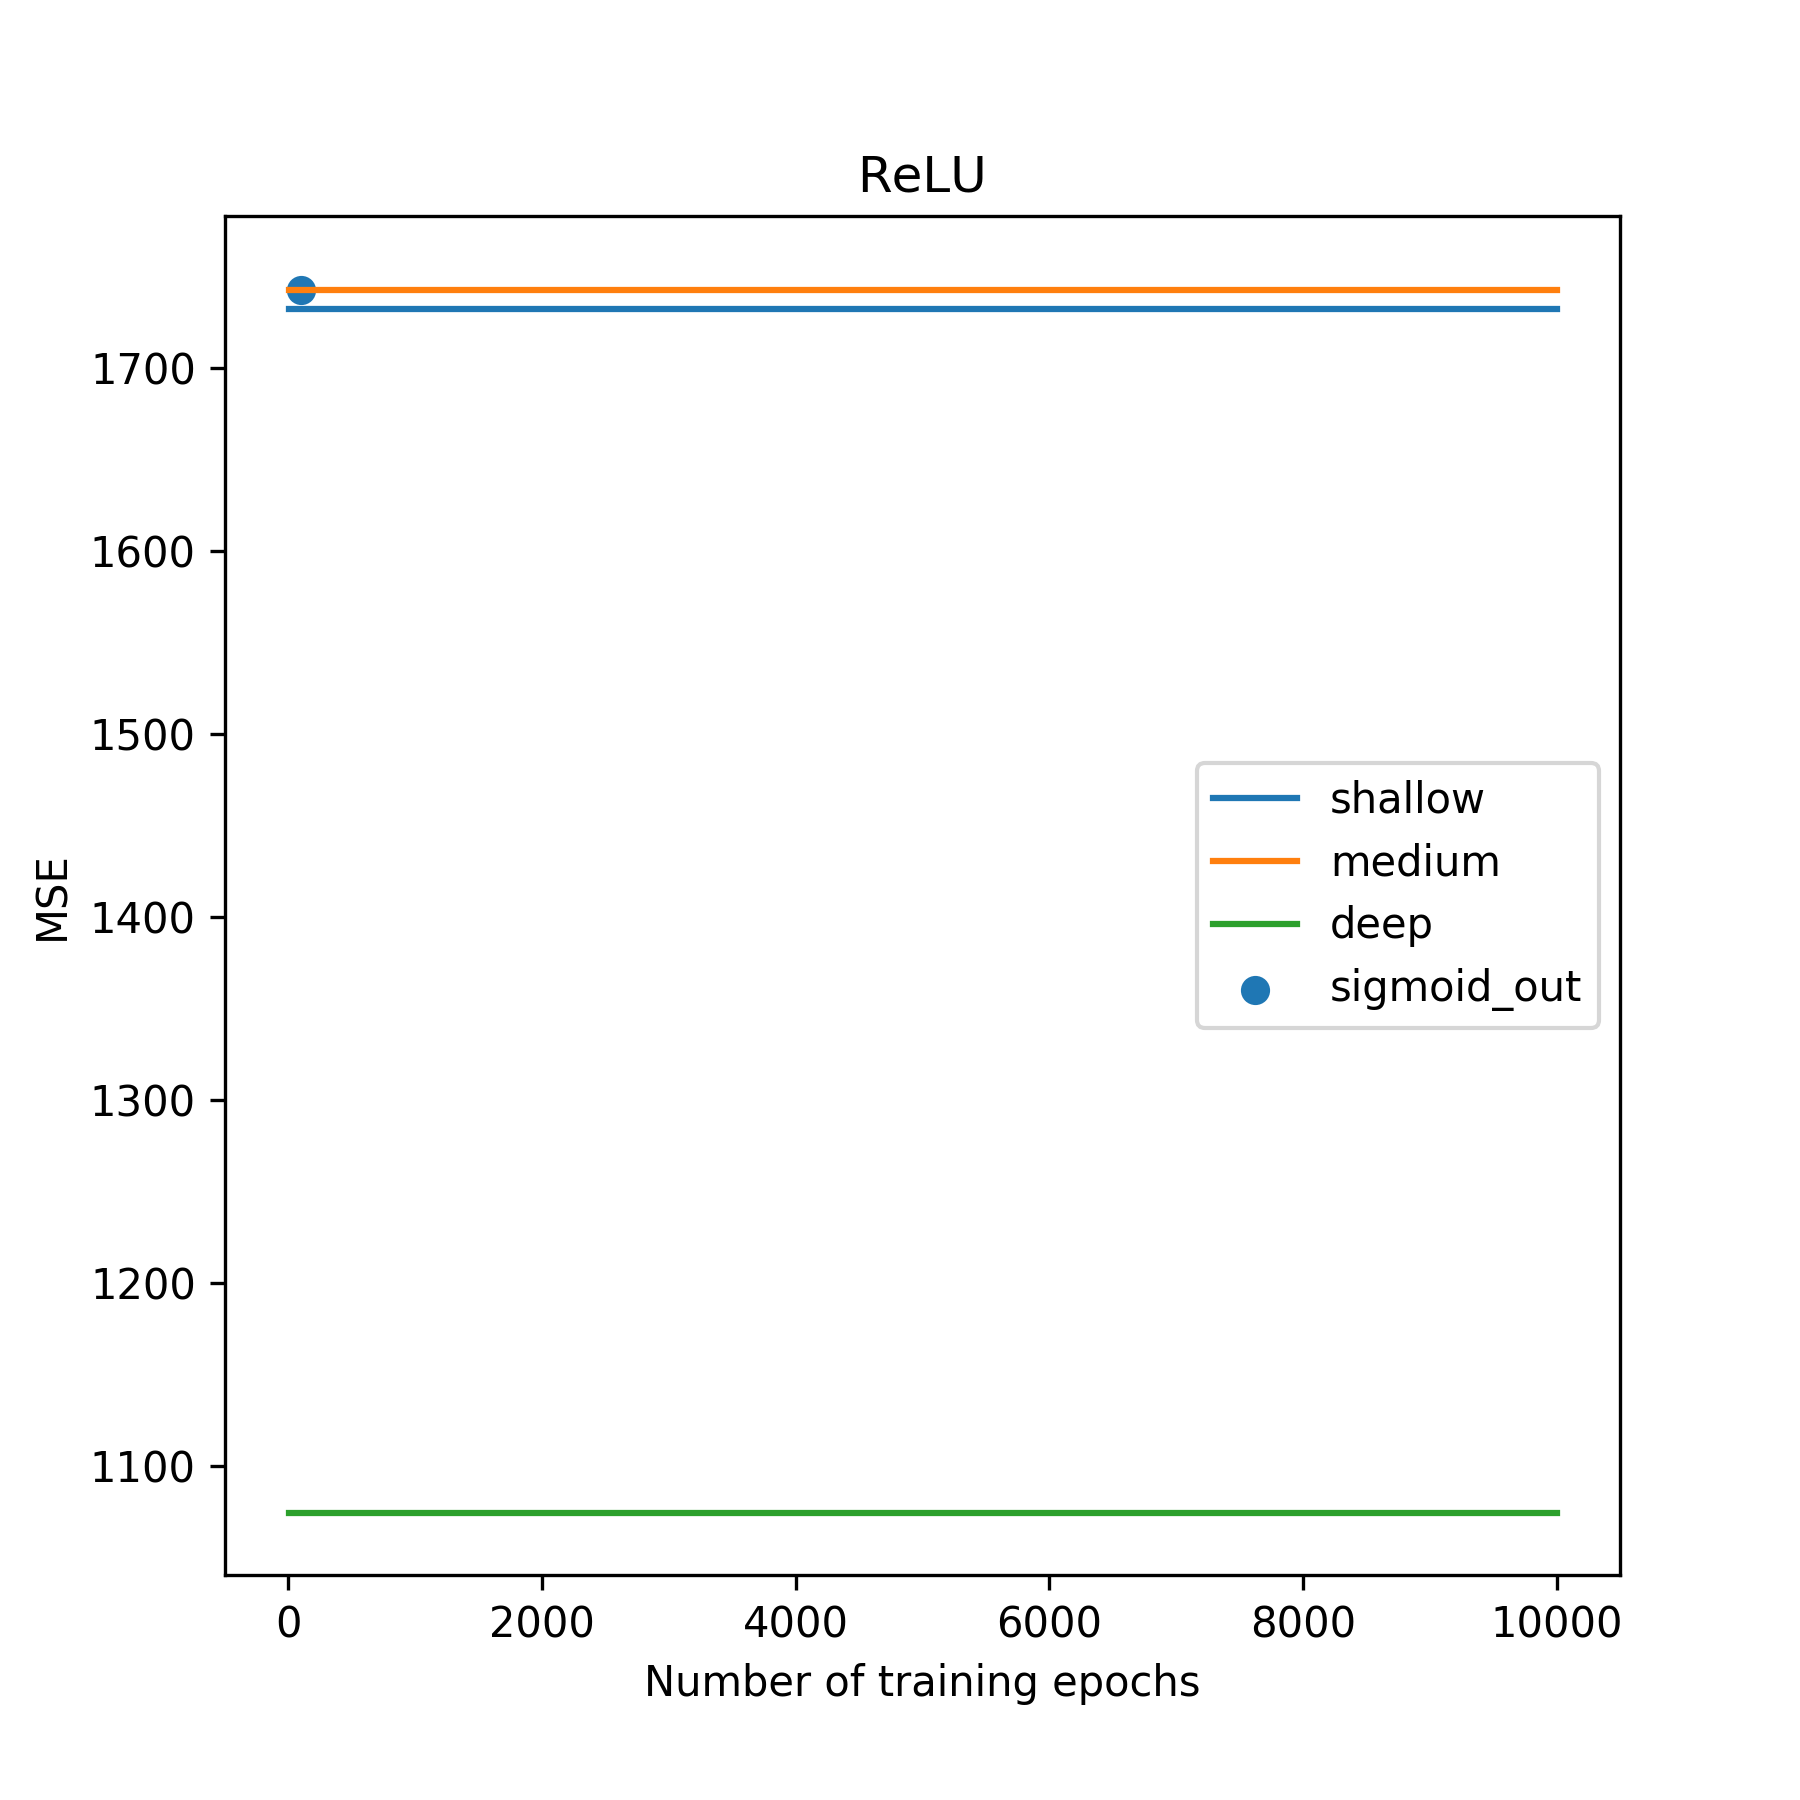
\includegraphics[width=0.7\textwidth]{../images/aenn_results_relu.png}
\caption{Mean-square error of ReLU activation AENN across training periods.}
\label{aenn_relu}
\end{figure}

\section{Conclusions}
\begin{itemize}
\item Autoencoders with logistic activation performed the best at dimensionality reduction (according to our regression mean-squared error metric), followed by regular principal-components analysis.
\item Neural networks with only ReLU activations do not perform well for dimensionality reduction, compared to other techniques we looked at.
\item For the architectures we studied, varying the number of training epochs did not change the mean-squared error. 
\item Neither combining layers with different activation functions (input and hidden ReLU and sigmoid output), nor adding symmetric decoding layers improved autoencoder performance.
\end{itemize}
\section{Future work}

There are a number of ways this work can be extended. As dicussed above, we could use alternate encoding schemes for the free-text data. Additional lines of inquiry involve either different neural-network architectures, different loss functions, or alternative dimensionality reduction techniques.

We could have used regression mean-squared error as the loss function when training neural networks, but there is not a clear analog of this when doing principal-components analysis, so we opted to simply force the decoded output to be as close as possible to the unencoded input.

Further, we had hoped to compare the methods discussed to another technique called t-Distributed Stochastic Neighbor Embedding (t-SNE) [9]. Other uses of this technique, which specifically targets two- or three-dimensional representations of high-dimensional data. These techniques exist on a spectrum of stochasticity: PCA is deterministic, while autoencoders have stochastic elements, and t-SNE is completely stochastic and very sensitive to hyperparameter tuning.

\section*{References}
\small

[1] Kramer, Mark A. (1991). "Nonlinear principal component analysis using autoassociative neural networks" {\it AIChE Journal}. 37 (2): 233–243. doi:10.1002/aic.690370209.

[2] Van der Maaten, L., Postma, E. (2009). Dimensionality Reduction: A Comparative Review. {\it Accessed at \verb+https://lvdmaaten.github.io/publications/papers/TR_Dimensionality\_Reduction\_Review\_2009.pdf+}. Last accessed Dec 19, 2019.

[3] Elden, L. (2007). {\it Matrix Methods in Data Mining and Pattern Recognition}, pp. 66. Philadelphia, PA:  Society for Industrial and Applied Mathematics.

[4] Hinton, G.E. \& Salakhutdinov, R.R. Reducing the dimensionality of data with neural networks. {\it Science}, 313(5786):504–507, 2006.

[5] Hinton GE, Krizhevsky A, Wang SD. Transforming auto-encoders. In International Conference on Artificial Neural Networks 2011 Jun 14 (pp. 44-51). Springer, Berlin, Heidelberg.

[6] https://www.kaggle.com/theonenamedtoby/auto-encoder-in-raw-numpy/data

[7] Wine Reviews (2017). {\it Accessed at https://kaggle.com/zynicide/wine-reviews}. Last accessed Dec 2, 2019.

[8] Mikolov, T., Chen, K., Corrado, G. \& Dean, J. (2013) Efficient Estimation of Word Representations in Vector Space. {\it Accessed at https://arXiv:1301.3781}. Last accessed Dec 10, 2019.

[9] L.J.P. van der Maaten and G.E. Hinton. Visualizing High-Dimensional Data Using t-SNE. Journal of Machine Learning Research 9(Nov):2579-2605, 2008.





% \section{Original}

% NeurIPS requires electronic submissions.  The electronic submission site is
% \begin{center}
%   \url{https://cmt.research.microsoft.com/NeurIPS2019/}
% \end{center}

% Please read the instructions below carefully and follow them faithfully.

% \subsection{Style}

% Papers to be submitted to NeurIPS 2019 must be prepared according to the
% instructions presented here. Papers may only be up to eight pages long,
% including figures. Additional pages \emph{containing only acknowledgments and/or
%   cited references} are allowed. Papers that exceed eight pages of content
% (ignoring references) will not be reviewed, or in any other way considered for
% presentation at the conference.

% The margins in 2019 are the same as since 2007, which allow for $\sim$$15\%$
% more words in the paper compared to earlier years.

% Authors are required to use the NeurIPS \LaTeX{} style files obtainable at the
% NeurIPS website as indicated below. Please make sure you use the current files
% and not previous versions. Tweaking the style files may be grounds for
% rejection.

% \subsection{Retrieval of style files}

% The style files for NeurIPS and other conference information are available on
% the World Wide Web at
% \begin{center}
%   \url{http://www.neurips.cc/}
% \end{center}
% The file \verb+neurips_2019.pdf+ contains these instructions and illustrates the
% various formatting requirements your NeurIPS paper must satisfy.

% The only supported style file for NeurIPS 2019 is \verb+neurips_2019.sty+,
% rewritten for \LaTeXe{}.  \textbf{Previous style files for \LaTeX{} 2.09,
%   Microsoft Word, and RTF are no longer supported!}

% The \LaTeX{} style file contains three optional arguments: \verb+final+, which
% creates a camera-ready copy, \verb+preprint+, which creates a preprint for
% submission to, e.g., arXiv, and \verb+nonatbib+, which will not load the
% \verb+natbib+ package for you in case of package clash.

% \paragraph{Preprint option}
% If you wish to post a preprint of your work online, e.g., on arXiv, using the
% NeurIPS style, please use the \verb+preprint+ option. This will create a
% nonanonymized version of your work with the text ``Preprint. Work in progress.''
% in the footer. This version may be distributed as you see fit. Please \textbf{do
%   not} use the \verb+final+ option, which should \textbf{only} be used for
% papers accepted to NeurIPS.

% At submission time, please omit the \verb+final+ and \verb+preprint+
% options. This will anonymize your submission and add line numbers to aid
% review. Please do \emph{not} refer to these line numbers in your paper as they
% will be removed during generation of camera-ready copies.

% The file \verb+neurips_2019.tex+ may be used as a ``shell'' for writing your
% paper. All you have to do is replace the author, title, abstract, and text of
% the paper with your own.

% The formatting instructions contained in these style files are summarized in
% Sections \ref{gen_inst}, \ref{headings}, and \ref{others} below.

% \section{General formatting instructions}
% \label{gen_inst}

% The text must be confined within a rectangle 5.5~inches (33~picas) wide and
% 9~inches (54~picas) long. The left margin is 1.5~inch (9~picas).  Use 10~point
% type with a vertical spacing (leading) of 11~points.  Times New Roman is the
% preferred typeface throughout, and will be selected for you by default.
% Paragraphs are separated by \nicefrac{1}{2}~line space (5.5 points), with no
% indentation.

% The paper title should be 17~point, initial caps/lower case, bold, centered
% between two horizontal rules. The top rule should be 4~points thick and the
% bottom rule should be 1~point thick. Allow \nicefrac{1}{4}~inch space above and
% below the title to rules. All pages should start at 1~inch (6~picas) from the
% top of the page.

% For the final version, authors' names are set in boldface, and each name is
% centered above the corresponding address. The lead author's name is to be listed
% first (left-most), and the co-authors' names (if different address) are set to
% follow. If there is only one co-author, list both author and co-author side by
% side.

% Please pay special attention to the instructions in Section \ref{others}
% regarding figures, tables, acknowledgments, and references.

% \section{Headings: first level}
% \label{headings}

% All headings should be lower case (except for first word and proper nouns),
% flush left, and bold.

% First-level headings should be in 12-point type.

% \subsection{Headings: second level}

% Second-level headings should be in 10-point type.

% \subsubsection{Headings: third level}

% Third-level headings should be in 10-point type.

% \paragraph{Paragraphs}

% There is also a \verb+\paragraph+ command available, which sets the heading in
% bold, flush left, and inline with the text, with the heading followed by 1\,em
% of space.

% \section{Citations, figures, tables, references}
% \label{others}

% These instructions apply to everyone.

% \subsection{Citations within the text}

% The \verb+natbib+ package will be loaded for you by default.  Citations may be
% author/year or numeric, as long as you maintain internal consistency.  As to the
% format of the references themselves, any style is acceptable as long as it is
% used consistently.

% The documentation for \verb+natbib+ may be found at
% \begin{center}
%   \url{http://mirrors.ctan.org/macros/latex/contrib/natbib/natnotes.pdf}
% \end{center}
% Of note is the command \verb+\citet+, which produces citations appropriate for
% use in inline text.  For example,
% \begin{verbatim}
%    \citet{hasselmo} investigated\dots
% \end{verbatim}
% produces
% \begin{quote}
%   Hasselmo, et al.\ (1995) investigated\dots
% \end{quote}

% If you wish to load the \verb+natbib+ package with options, you may add the
% following before loading the \verb+neurips_2019+ package:
% \begin{verbatim}
%    \PassOptionsToPackage{options}{natbib}
% \end{verbatim}

% If \verb+natbib+ clashes with another package you load, you can add the optional
% argument \verb+nonatbib+ when loading the style file:
% \begin{verbatim}
%    \usepackage[nonatbib]{neurips_2019}
% \end{verbatim}

% As submission is double blind, refer to your own published work in the third
% person. That is, use ``In the previous work of Jones et al.\ [4],'' not ``In our
% previous work [4].'' If you cite your other papers that are not widely available
% (e.g., a journal paper under review), use anonymous author names in the
% citation, e.g., an author of the form ``A.\ Anonymous.''

% \subsection{Footnotes}

% Footnotes should be used sparingly.  If you do require a footnote, indicate
% footnotes with a number\footnote{Sample of the first footnote.} in the
% text. Place the footnotes at the bottom of the page on which they appear.
% Precede the footnote with a horizontal rule of 2~inches (12~picas).

% Note that footnotes are properly typeset \emph{after} punctuation
% marks.\footnote{As in this example.}

% \subsection{Figures}

% \begin{figure}
%   \centering
%   \fbox{\rule[-.5cm]{0cm}{4cm} \rule[-.5cm]{4cm}{0cm}}
%   \caption{Sample figure caption.}
% \end{figure}

% All artwork must be neat, clean, and legible. Lines should be dark enough for
% purposes of reproduction. The figure number and caption always appear after the
% figure. Place one line space before the figure caption and one line space after
% the figure. The figure caption should be lower case (except for first word and
% proper nouns); figures are numbered consecutively.

% You may use color figures.  However, it is best for the figure captions and the
% paper body to be legible if the paper is printed in either black/white or in
% color.

% \subsection{Tables}

% All tables must be centered, neat, clean and legible.  The table number and
% title always appear before the table.  See Table~\ref{sample-table}.

% Place one line space before the table title, one line space after the
% table title, and one line space after the table. The table title must
% be lower case (except for first word and proper nouns); tables are
% numbered consecutively.

% Note that publication-quality tables \emph{do not contain vertical rules.} We
% strongly suggest the use of the \verb+booktabs+ package, which allows for
% typesetting high-quality, professional tables:
% \begin{center}
%   \url{https://www.ctan.org/pkg/booktabs}
% \end{center}
% This package was used to typeset Table~\ref{sample-table}.

% \begin{table}
%   \caption{Sample table title}
%   \label{sample-table}
%   \centering
%   \begin{tabular}{lll}
%     \toprule
%     \multicolumn{2}{c}{Part}                   \\
%     \cmidrule(r){1-2}
%     Name     & Description     & Size ($\mu$m) \\
%     \midrule
%     Dendrite & Input terminal  & $\sim$100     \\
%     Axon     & Output terminal & $\sim$10      \\
%     Soma     & Cell body       & up to $10^6$  \\
%     \bottomrule
%   \end{tabular}
% \end{table}

% \section{Final instructions}

% Do not change any aspects of the formatting parameters in the style files.  In
% particular, do not modify the width or length of the rectangle the text should
% fit into, and do not change font sizes (except perhaps in the
% \textbf{References} section; see below). Please note that pages should be
% numbered.

% \section{Preparing PDF files}

% Please prepare submission files with paper size ``US Letter,'' and not, for
% example, ``A4.''

% Fonts were the main cause of problems in the past years. Your PDF file must only
% contain Type 1 or Embedded TrueType fonts. Here are a few instructions to
% achieve this.

% \begin{itemize}

% \item You should directly generate PDF files using \verb+pdflatex+.

% \item You can check which fonts a PDF files uses.  In Acrobat Reader, select the
%   menu Files$>$Document Properties$>$Fonts and select Show All Fonts. You can
%   also use the program \verb+pdffonts+ which comes with \verb+xpdf+ and is
%   available out-of-the-box on most Linux machines.

% \item The IEEE has recommendations for generating PDF files whose fonts are also
%   acceptable for NeurIPS. Please see
%   \url{http://www.emfield.org/icuwb2010/downloads/IEEE-PDF-SpecV32.pdf}

% \item \verb+xfig+ "patterned" shapes are implemented with bitmap fonts.  Use
%   "solid" shapes instead.

% \item The \verb+\bbold+ package almost always uses bitmap fonts.  You should use
%   the equivalent AMS Fonts:
% \begin{verbatim}
%    \usepackage{amsfonts}
% \end{verbatim}
% followed by, e.g., \verb+\mathbb{R}+, \verb+\mathbb{N}+, or \verb+\mathbb{C}+
% for $\mathbb{R}$, $\mathbb{N}$ or $\mathbb{C}$.  You can also use the following
% workaround for reals, natural and complex:
% \begin{verbatim}
%    \newcommand{\RR}{I\!\!R} %real numbers
%    \newcommand{\Nat}{I\!\!N} %natural numbers
%    \newcommand{\CC}{I\!\!\!\!C} %complex numbers
% \end{verbatim}
% Note that \verb+amsfonts+ is automatically loaded by the \verb+amssymb+ package.

% \end{itemize}

% If your file contains type 3 fonts or non embedded TrueType fonts, we will ask
% you to fix it.

% \subsection{Margins in \LaTeX{}}

% Most of the margin problems come from figures positioned by hand using
% \verb+\special+ or other commands. We suggest using the command
% \verb+\includegraphics+ from the \verb+graphicx+ package. Always specify the
% figure width as a multiple of the line width as in the example below:
% \begin{verbatim}
%    \usepackage[pdftex]{graphicx} ...
%    \includegraphics[width=0.8\linewidth]{myfile.pdf}
% \end{verbatim}
% See Section 4.4 in the graphics bundle documentation
% (\url{http://mirrors.ctan.org/macros/latex/required/graphics/grfguide.pdf})

% A number of width problems arise when \LaTeX{} cannot properly hyphenate a
% line. Please give LaTeX hyphenation hints using the \verb+\-+ command when
% necessary.

% \subsubsection*{Acknowledgments}

% Use unnumbered third level headings for the acknowledgments. All acknowledgments
% go at the end of the paper. Do not include acknowledgments in the anonymized
% submission, only in the final paper.

% \section*{References}

% References follow the acknowledgments. Use unnumbered first-level heading for
% the references. Any choice of citation style is acceptable as long as you are
% consistent. It is permissible to reduce the font size to \verb+small+ (9 point)
% when listing the references. {\bf Remember that you can use more than eight
%   pages as long as the additional pages contain \emph{only} cited references.}
% \medskip

% \small

% [1] Alexander, J.A.\ \& Mozer, M.C.\ (1995) Template-based algorithms for
% connectionist rule extraction. In G.\ Tesauro, D.S.\ Touretzky and T.K.\ Leen
% (eds.), {\it Advances in Neural Information Processing Systems 7},
% pp.\ 609--616. Cambridge, MA: MIT Press.

% [2] Bower, J.M.\ \& Beeman, D.\ (1995) {\it The Book of GENESIS: Exploring
%   Realistic Neural Models with the GEneral NEural SImulation System.}  New York:
% TELOS/Springer--Verlag.

% [3] Hasselmo, M.E., Schnell, E.\ \& Barkai, E.\ (1995) Dynamics of learning and
% recall at excitatory recurrent synapses and cholinergic modulation in rat
% hippocampal region CA3. {\it Journal of Neuroscience} {\bf 15}(7):5249-5262.

\end{document}
